\documentclass[11pt,letterpaper]{article}
\usepackage{graphicx}
\usepackage{blindtext}
\usepackage{geometry}
\usepackage{fancyhdr}
\usepackage{tikz}
\usepackage{pgfplots}




\pagestyle{fancy}
\fancyhf{}
\rhead{\small {© 2022 All Rights Reserved, Aiden Rosenberg}}
\rfoot{Page \thepage}


\title{Statue in the Headlights}
\author{Aiden Rosenberg}
\date{August 2022}

\begin{document}
\maketitle
\section{Discription}
A car is traveling at night along a highway shaped like a parabola with its vertex at the origin. The car starts at a point 100 miles west and 100 miles north of the origin and travels in an easterly direction. There is a statue located 100 miles east and 50 miles north. At what point on the highway will the car's headlights illuminate the statue? 

\subsection{Graphical Analysis}
\begin{center}
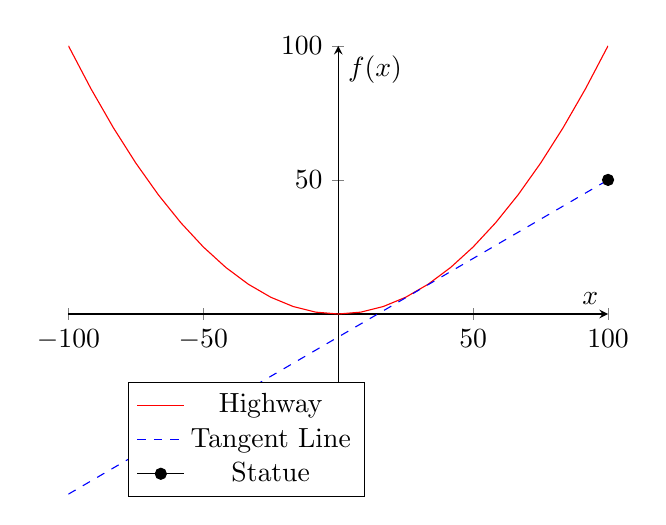
\begin{tikzpicture}
\begin{axis}[
    axis lines = center,
    xlabel = \(x\),
    ylabel = {\(f(x)\)},
    legend style={at={(0.55,0.25)}}
    ]
\addplot [
    domain=-100:100, 
      range=0:100
    samples=100, 
    color=red,
]
{0.01*\x^2};
\addlegendentry{Highway}
%Here the blue parabola is defined
\addplot [
    domain=-100:100, 
    range=0:100
    samples=100,
    color=blue, dashed
]
{(2-sqrt(2))*(x-100) + 50};
\addlegendentry{Tangent Line}
%Here the blue parabola is defined
\addplot [color=black,mark=*]
    coordinates {
    (100,50)
    };
\addlegendentry{Statue}
\end{axis}
\end{tikzpicture}
\end{center}
\newpage

\subsection{Algebraic Solution}

$$f(x)=ax^2$$
$$f(-100)=100=a(-100)^2\Longrightarrow a=\frac{1}{100} \therefore f(x)=\frac{x^2}{100}$$
$$f'(x)=\frac{dy}{dy}(\frac{x^2}{100})=\frac{x}{50} $$ 
$$y-50=\frac{x}{50}(x-100)$$ 
$$y=\frac{x^2}{50}-2x+50$$
$$\frac{x^2}{50}-2x+50=\frac{x^2}{100}$$
$$0=x^2-200x+5000$$
$$x=\frac{200\pm\sqrt{(200)^2-4(5000)}}{2}$$
$$\Longrightarrow x= -50(\sqrt{2}-2) \approx 29.28 $$
$$\Longrightarrow x= 50(\sqrt{2}+2) \approx 170.71 \, \textit{This solution is only true when the tailights face the point}$$ 
$$f(x)\bigg\rvert_{x=-50(\sqrt{2}-2)}=-50(2\sqrt{2}-3) \approx 8.57$$

\subsection{Solution}
When the car is approximately $29.28$ metres north and $8.57$ metres east of the origin the car's headlights will illuminate the statues.

\end{document}

